%Copyright 2014 Jean-Philippe Eisenbarth
%This program is free software: you can 
%redistribute it and/or modify it under the terms of the GNU General Public 
%License as published by the Free Software Foundation, either version 3 of the 
%License, or (at your option) any later version.
%This program is distributed in the hope that it will be useful,but WITHOUT ANY 
%WARRANTY; without even the implied warranty of MERCHANTABILITY or FITNESS FOR A 
%PARTICULAR PURPOSE. See the GNU General Public License for more details.
%You should have received a copy of the GNU General Public License along with 
%this program.  If not, see <http://www.gnu.org/licenses/>.

%Based on the code of Yiannis Lazarides
%http://tex.stackexchange.com/questions/42602/software-requirements-specification-with-latex
%http://tex.stackexchange.com/users/963/yiannis-lazarides
%Also based on the template of Karl E. Wiegers
%http://www.se.rit.edu/~emad/teaching/slides/srs_template_sep14.pdf
%http://karlwiegers.com
\documentclass{scrreprt}
\usepackage{listings}
\usepackage{underscore}
\usepackage[bookmarks=true]{hyperref}
\usepackage[utf8]{inputenc}
\usepackage[english]{babel}
\usepackage{CJKutf8}
\usepackage{graphicx}
\usepackage{float}


\hypersetup{
    bookmarks=false,    % show bookmarks bar?
    pdftitle={Software Requirement Specification},    % title
    pdfauthor={Jean-Philippe Eisenbarth},                     % author
    pdfsubject={TeX and LaTeX},                        % subject of the document
    pdfkeywords={TeX, LaTeX, graphics, images}, % list of keywords
    colorlinks=true,       % false: boxed links; true: colored links
    linkcolor=blue,       % color of internal links
    citecolor=black,       % color of links to bibliography
    filecolor=black,        % color of file links
    urlcolor=purple,        % color of external links
    linktoc=page            % only page is linked
}%
\def\myversion{1.0 }
\date{}
%\title
\usepackage{hyperref}
\begin{document}
\begin{CJK}{UTF8}{bkai}
\begin{flushright}
    \rule{16cm}{5pt}\vskip1cm
    \begin{bfseries}
        \Huge{SOFTWARE REQUIREMENTS\\ SPECIFICATION}\\
        \vspace{1.9cm}
        for\\
        \vspace{1.9cm}
        $<$FinGer Shopping$>$\\
        \vspace{1.9cm}
        \LARGE{Version \myversion approved}\\
        \vspace{1.9cm}
        Prepared by $<$Rl$>$\\
        \vspace{1.9cm}
        $<$第11組$>$\\
        \vspace{1.9cm}
        \today\\
    \end{bfseries}
\end{flushright}

\tableofcontents


\chapter*{Revision History}

\begin{center}
    \begin{tabular}{|c|c|c|c|}
        \hline
	    Name & Date & Reason For Changes & Version\\
        \hline
	    21 & 22 & 23 & 24\\
        \hline
	    31 & 32 & 33 & 34\\
        \hline
    \end{tabular}
\end{center}

\chapter{介紹}

\section{目的}
\qquad FinGer shopping由human to human為核心出發,開發出一套小型的買賣交易系統。

\section{Document Conventions}
$<$Describe any standards or typographical conventions that were followed when 
writing this SRS, such as fonts or highlighting that have special significance.  
For example, state whether priorities  for higher-level requirements are assumed 
to be inherited by detailed requirements, or whether every requirement statement 
is to have its own priority.$>$

\section{Intended Audience and Reading Suggestions}
$<$Describe the different types of reader that the document is intended for, 
such as developers, project managers, marketing staff, users, testers, and 
documentation writers. Describe what the rest of this SRS contains and how it is 
organized. Suggest a sequence for reading the document, beginning with the 
overview sections and proceeding through the sections that are most pertinent to 
each reader type.$>$

\section{Project Scope}
$<$Provide a short description of the software being specified and its purpose, 
including relevant benefits, objectives, and goals. Relate the software to 
corporate goals or business strategies. If a separate vision and scope document 
is available, refer to it rather than duplicating its contents here.$>$

\section{References}
$<$List any other documents or Web addresses to which this SRS refers. These may 
include user interface style guides, contracts, standards, system requirements 
specifications, use case documents, or a vision and scope document. Provide 
enough information so that the reader could access a copy of each reference, 
including title, author, version number, date, and source or location.$>$


\chapter{產品描述}

\section{產品願景}
\qquad 在這個網路蓬勃發展的時代,人民對於使用網路可以說是隨手可得。而藉由我們實做出來的交易平台,希望能提供使用者一個簡單且便利買賣
的環境,不僅如此,買家可以輕鬆方便的擔任商品的供給與需求方,更提透明的評分機制,讓使用者可以清楚了解商品的資訊,建立一個隨時隨地都能隨手做買賣的輕鬆便利交易制度。

\section{產品功能}
\qquad FinGer Sopping是一套讓使用者可以同時具備商品的供給與需求方的交易平台。擔任賣家可以透過新增商品同時上傳該商品的圖片、制訂商品價格來銷售自己的商品,並且將會收到來自買方的訂單需求通知;而擔任買家的一方,則可以透過流覽商品來進行選購,若有疑問可以透過商品的評價、或是利用留言版的功能來詢問賣家或其他使用者相關的商品資訊,購買後還能做後續的商品狀態的追蹤。

\section{目標族群}
\qquad FinGer Sopping成立的宗旨主要為讓任何對銷售有興趣的使用者都能賣出自己的商品,平台提供賣方一個輕鬆便利提供商品的制度,達到人人都能在網路上當起大老闆;對於賣方則鎖定對網路相當熟悉的年輕人以及對於購買有強烈欲望的家庭主婦。

\section{開發環境}
\qquad 此專案主要由 C\# 中的 Window Form 來作開發環境,並且以 mongodb 做為資料庫,來儲存用戶的相關資料,成品說明則是由LaTex撰寫而成。

\section{程式架構}
\qquad 使用MongoDB做為資料庫,並統一用BaseDB作為存取資料庫的基礎,再依照各頁面不同的需求來新增不同的class,來在相對應的collection進行一個存取的動作。\\

\begin{figure}
	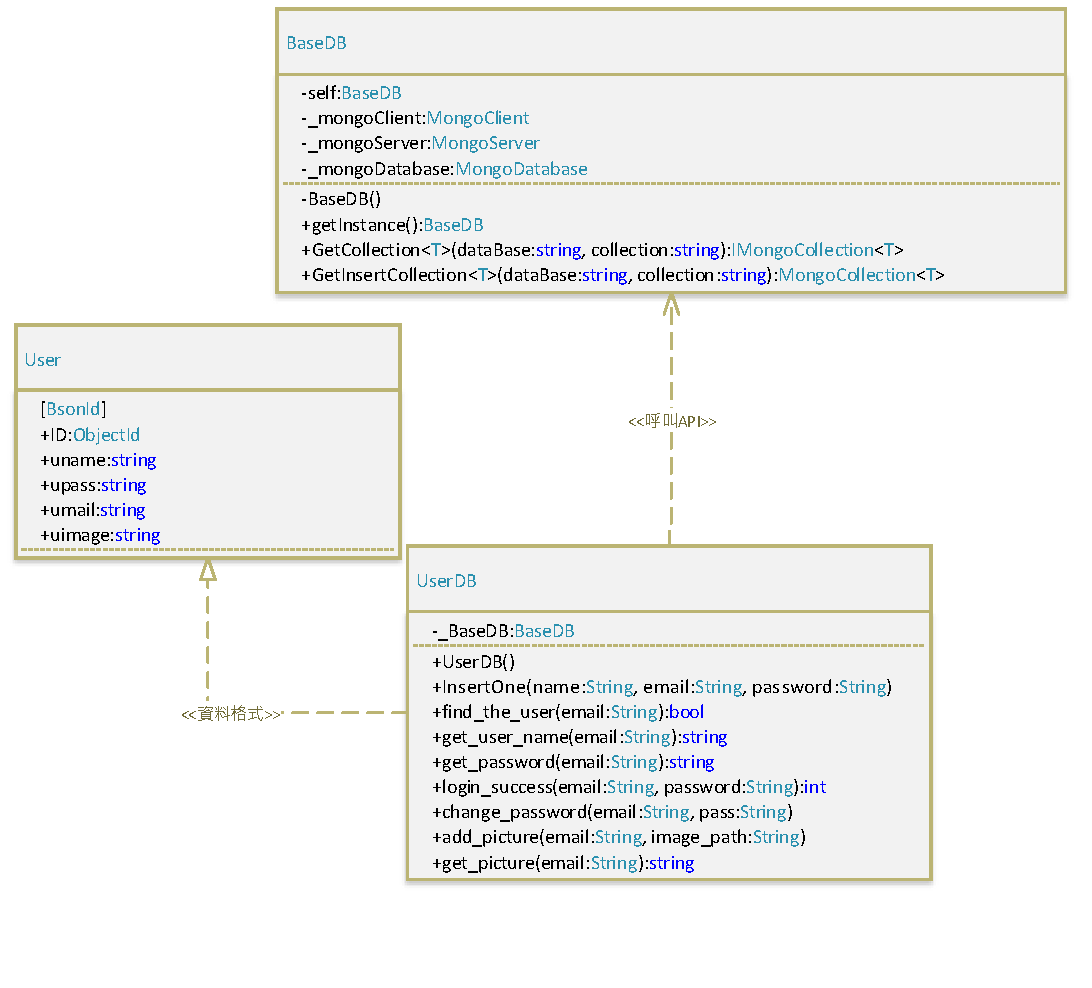
\includegraphics[width=\textwidth]{UserDB.pdf}
	\caption{UserDB用來處理新增、修改使用者登入到資料庫。}
\end{figure}

\begin{figure}
	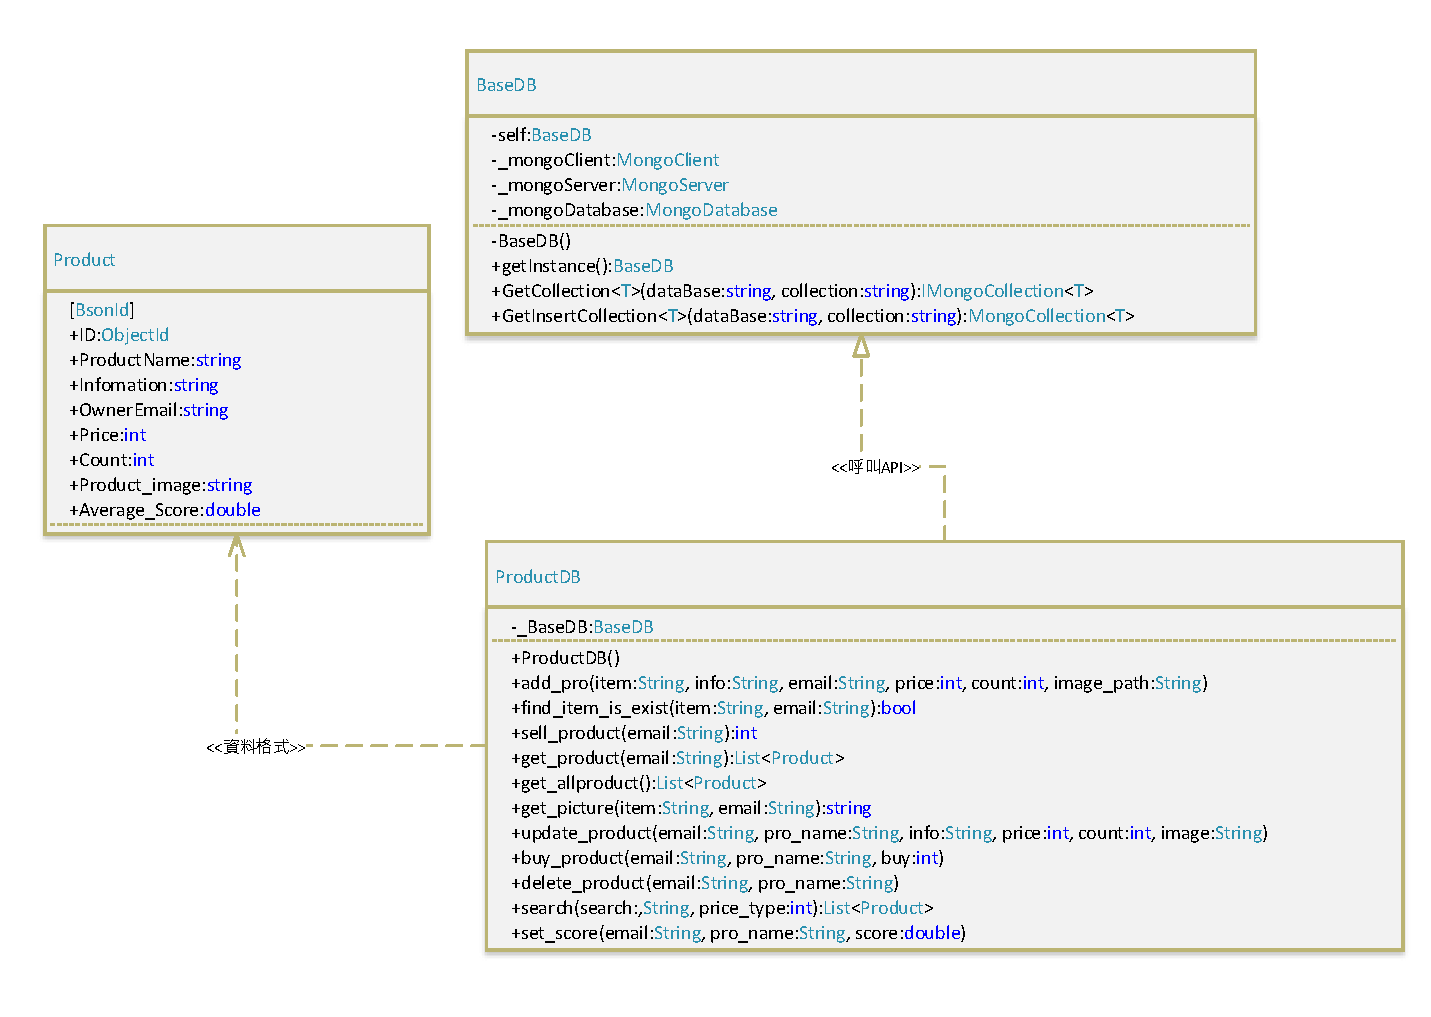
\includegraphics[width=\textwidth]{ProductDB.pdf}
	\caption{ProductDB用來對商品新增、修改、刪除。}
\end{figure}

\begin{figure}
	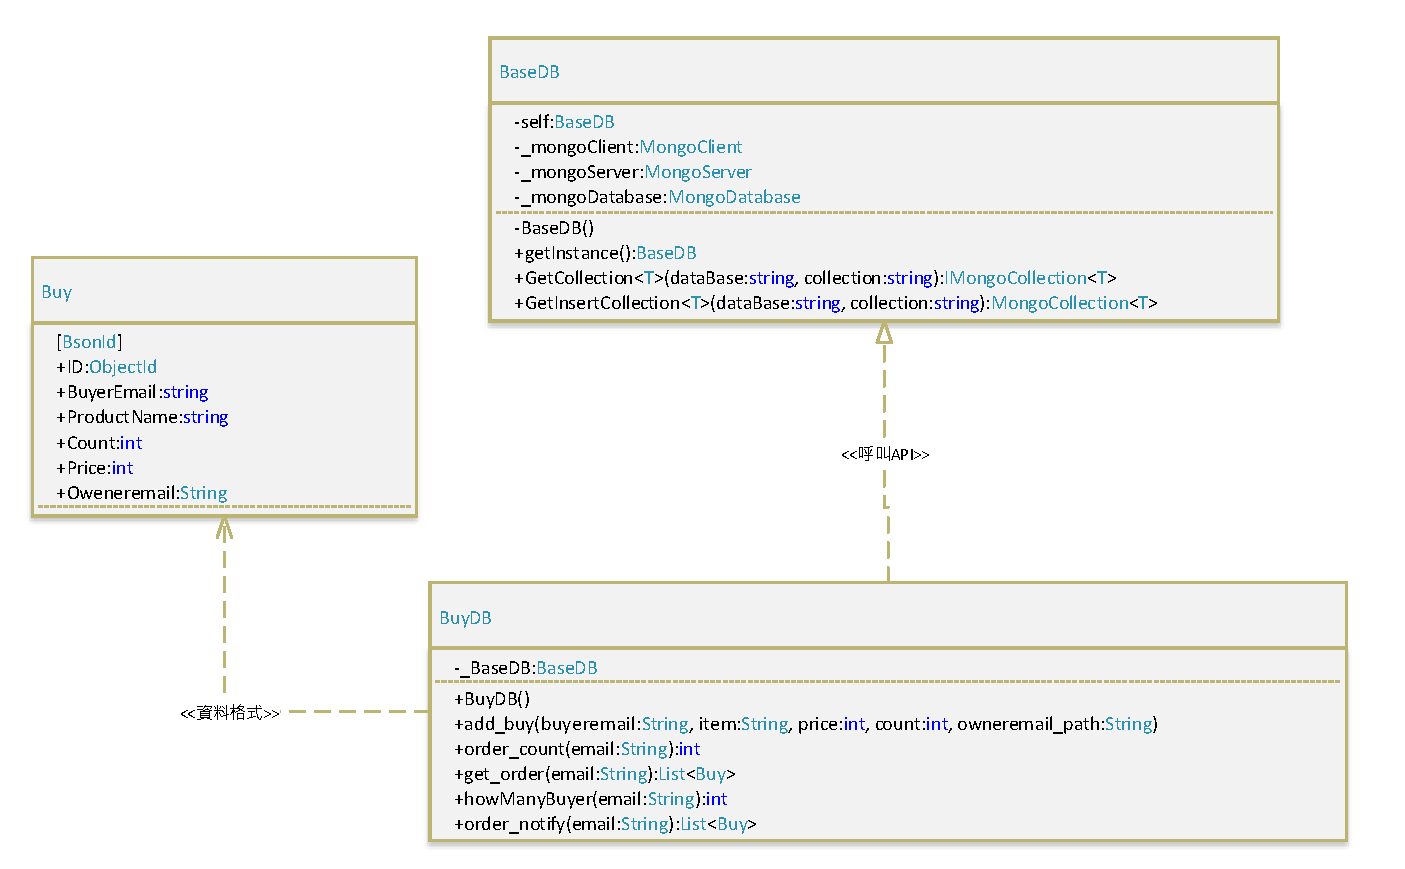
\includegraphics[width=\textwidth]{BuyDB.pdf}
	\caption{BuyDB用來對儲存商品購買紀錄。}
\end{figure}

\begin{figure}
	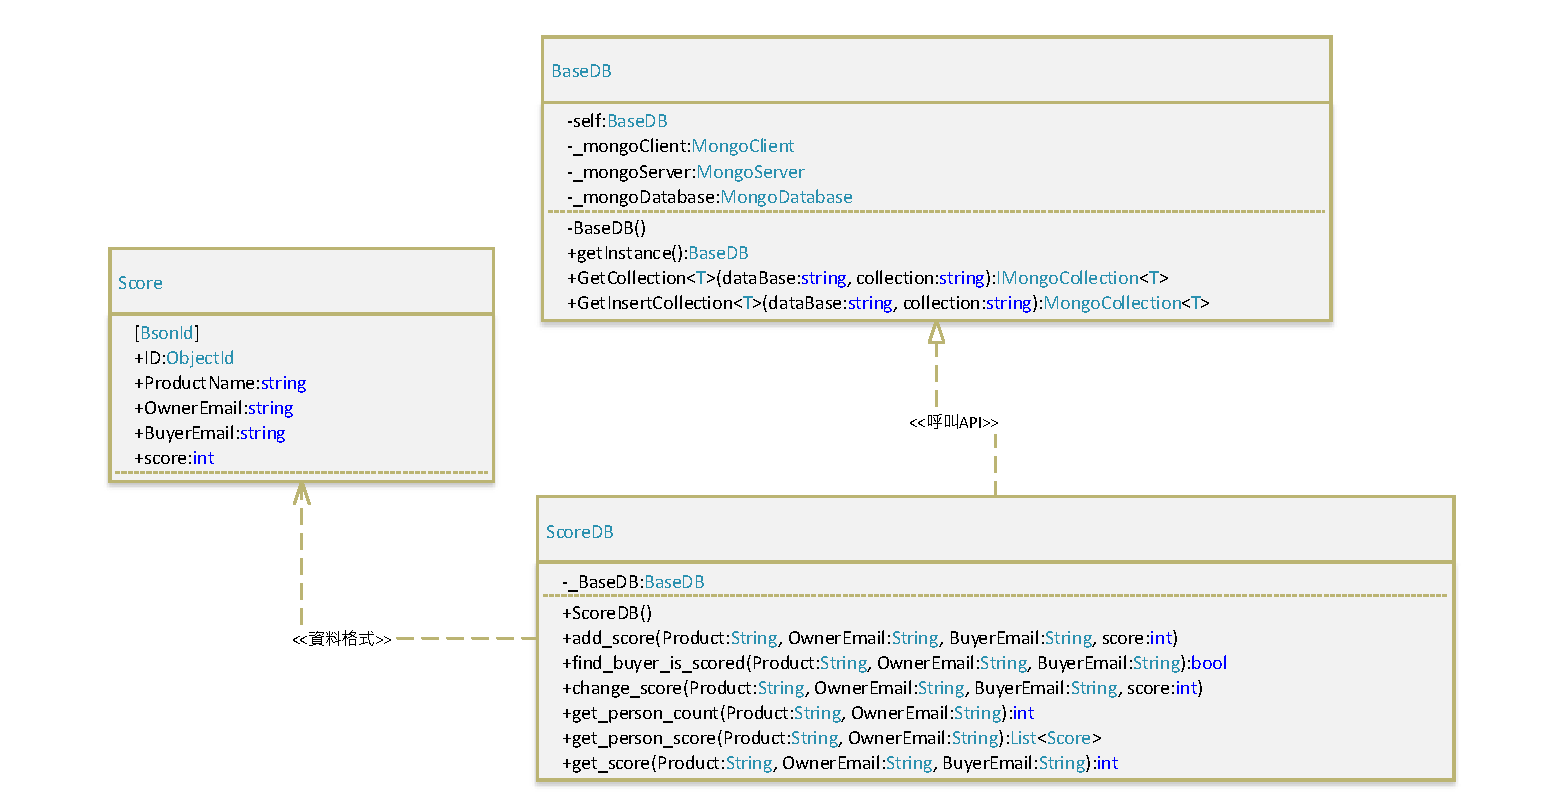
\includegraphics[width=\textwidth]{ScoreDB.pdf}
	\caption{ScoreDB用來紀錄不同使用者對商品的評分。}
\end{figure}

\begin{figure}
	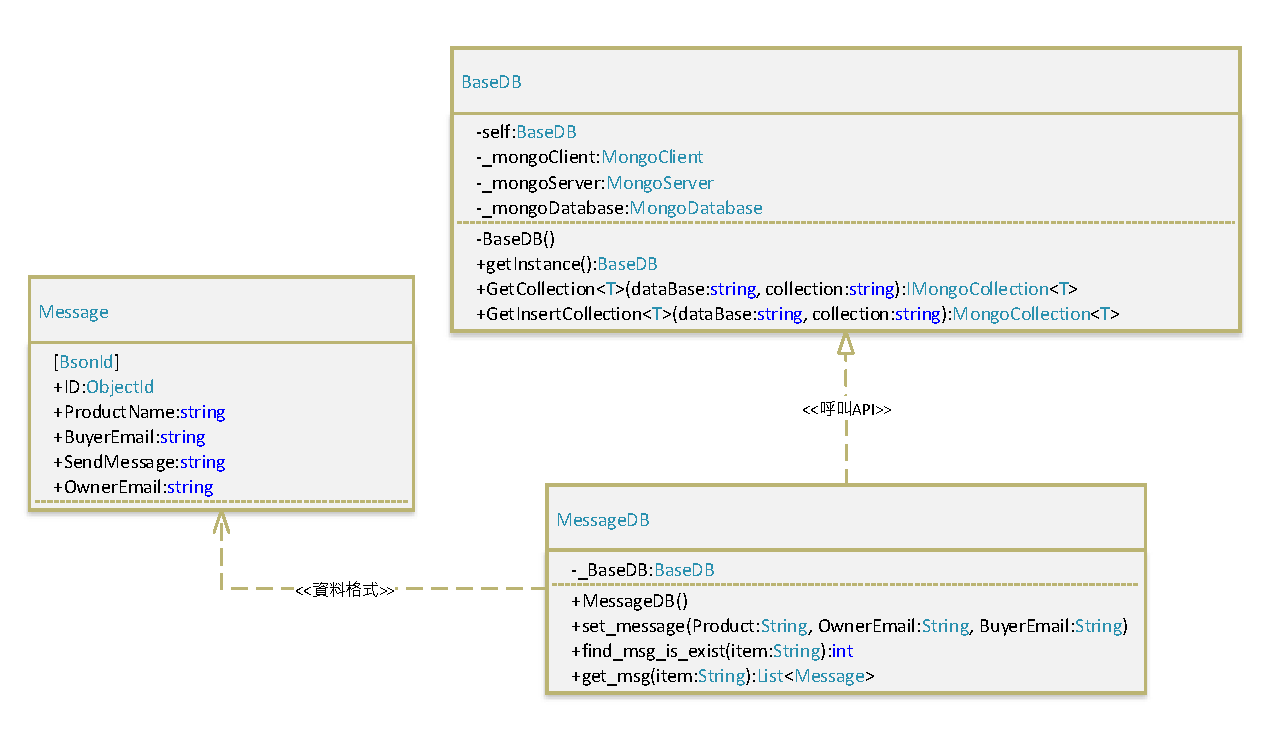
\includegraphics[width=\textwidth]{MessageDB.pdf}
	\caption{MessageDB用來紀錄不同商品使用者對其的留言。}
\end{figure}


\chapter{External Interface Requirements}

\section{User Interfaces}
\begin{figure}[h]
	\centering
	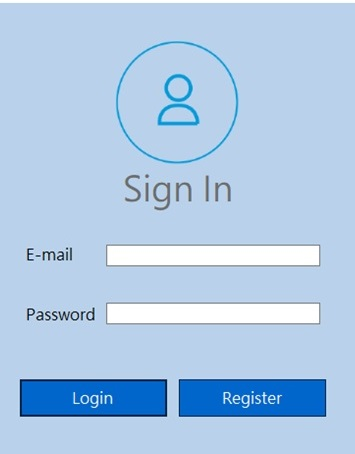
\includegraphics[width=0.33\textwidth]{signin.jpg}
	\caption{登入畫面。}
	\centering
	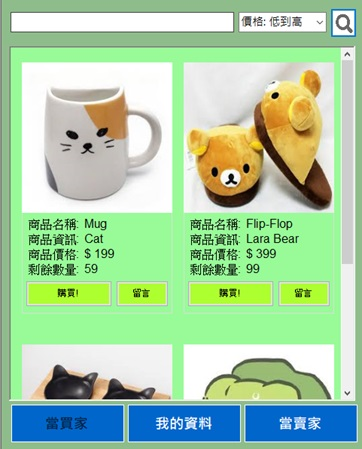
\includegraphics[width=0.33\textwidth]{search.jpg}
	\caption{登入後的頁面,會呈現目前可以買賣的商品。}
\end{figure}

\begin{figure}[t]
	\centering
	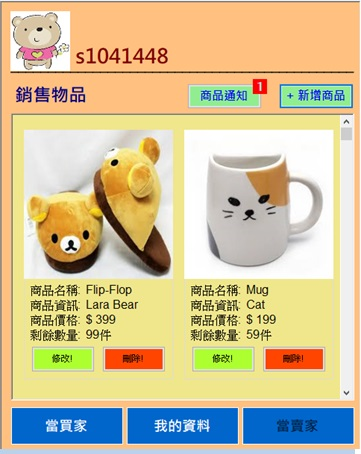
\includegraphics[width=0.45\textwidth]{note.jpg}
	\caption{賣家的畫面。}
	\centering
	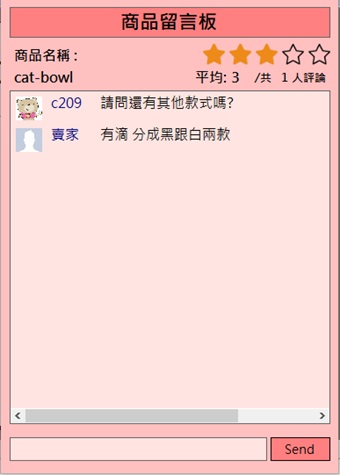
\includegraphics[width=0.45\textwidth]{star.jpg}
	\caption{商品留言和評分頁面。}
\end{figure}


\chapter{系統特色}
\section{輕鬆的購物方式}

\subsection{即時性}
\qquad 賣家可以在 FinGer Sopping 隨時新增商品,在有使用者購買其商品時,能提供即時的買賣資訊和通知;買家也可以隨時選取自己想要的商品進行購買,並且即時的追蹤商品的狀態。

\subsection{便利性}
\qquad 在任何有網路的地方,都能隨時當起買家和賣家,只要輕鬆按下一鍵,就能在賣家和買家之間能夠自由切換自己的角色。


\section{舒適的介面}

\subsection{暖色系的色彩}
\qquad 根據研究,由於受到色彩的視覺刺激,而在思維上有所影響。而我們在 FinGer Sopping 上大量採用暖色系的顏料,人類對於暖色系的色彩會感到興奮感,進而提升買家購買的慾望,而對於暖色系的色彩也比較不會對人類的視覺感到疲憊。

\section{產品資訊透明化}
\subsection{評分系統}
\qquad 藉由買家購買的感受度,來給商品評分,讓好的賣家能夠得到更多的回饋,也能讓使用者能夠挑選較優質的商品。

\subsection{留言板的設計}
\qquad 若買家對於商品存在任何疑問,可以透過 FinGer Sopping 提供使用者的留言版來詢問賣家產品的相關問題,也能讓其他想購買此商品的買家能夠在留言板上尋找相關的答案或給予相關的意見。

\chapter{Other Nonfunctional Requirements}

\section{Performance Requirements}
$<$If there are performance requirements for the product under various 
circumstances, state them here and explain their rationale, to help the 
developers understand the intent and make suitable design choices. Specify the 
timing relationships for real time systems. Make such requirements as specific 
as possible. You may need to state performance requirements for individual 
functional requirements or features.$>$

\section{Safety Requirements}
$<$Specify those requirements that are concerned with possible loss, damage, or 
harm that could result from the use of the product. Define any safeguards or 
actions that must be taken, as well as actions that must be prevented. Refer to 
any external policies or regulations that state safety issues that affect the 
product’s design or use. Define any safety certifications that must be 
satisfied.$>$

\section{Security Requirements}
$<$Specify any requirements regarding security or privacy issues surrounding use 
of the product or protection of the data used or created by the product. Define 
any user identity authentication requirements. Refer to any external policies or 
regulations containing security issues that affect the product. Define any 
security or privacy certifications that must be satisfied.$>$

\section{Software Quality Attributes}
$<$Specify any additional quality characteristics for the product that will be 
important to either the customers or the developers. Some to consider are: 
adaptability, availability, correctness, flexibility, interoperability, 
maintainability, portability, reliability, reusability, robustness, testability, 
and usability. Write these to be specific, quantitative, and verifiable when 
possible. At the least, clarify the relative preferences for various attributes, 
such as ease of use over ease of learning.$>$

\section{Business Rules}
$<$List any operating principles about the product, such as which individuals or 
roles can perform which functions under specific circumstances. These are not 
functional requirements in themselves, but they may imply certain functional 
requirements to enforce the rules.$>$


\chapter{Other Requirements}
$<$Define any other requirements not covered elsewhere in the SRS. This might 
include database requirements, internationalization requirements, legal 
requirements, reuse objectives for the project, and so on. Add any new sections 
that are pertinent to the project.$>$

\section{Appendix A: Glossary}
%see https://en.wikibooks.org/wiki/LaTeX/Glossary
$<$Define all the terms necessary to properly interpret the SRS, including 
acronyms and abbreviations. You may wish to build a separate glossary that spans 
multiple projects or the entire organization, and just include terms specific to 
a single project in each SRS.$>$

\section{Appendix B: Analysis Models}
$<$Optionally, include any pertinent analysis models, such as data flow 
diagrams, class diagrams, state-transition diagrams, or entity-relationship 
diagrams.$>$

\section{Appendix C: To Be Determined List}
$<$Collect a numbered list of the TBD (to be determined) references that remain 
in the SRS so they can be tracked to closure.$>$
\end{CJK}
\end{document}
